\documentclass[12pt,a4paper]{article}
\usepackage{amsmath, amssymb, geometry, booktabs, xcolor, hyperref,
            listings, pgfplots, tcolorbox, enumitem, fancyhdr, tikz, array}
\usepgfplotslibrary{fillbetween}
\geometry{margin=2.5cm}
\pgfplotsset{compat=1.18}
\tcbuselibrary{skins, breakable}

% Define custom environments
\newtcolorbox{curiositybox}[1][]{colback=yellow!10, colframe=orange!80, title=#1, breakable}
\newtcolorbox{infobox}[1][]{colback=blue!5, colframe=blue!60, title=#1, breakable}
\newtcolorbox{mistakebox}[1][]{colback=red!5, colframe=red!60, title=#1, breakable}
\newtcolorbox{learnbox}[1][]{colback=green!5, colframe=green!60, title=#1, breakable}

% Header and Footer
\pagestyle{fancy}
\fancyhf{}
\lhead{Rank, Index, Signature and Definite Forms}
\rhead{Unit 2 -- LAC}
\cfoot{\thepage}

% Document Title Setup
\title{\textbf{Rank, Index, Signature, and Definite Forms} \\ \large Unit 2 -- Eigenvalues, Eigenvectors, Diagonalization and Quadratic Forms}
\author{Department of Mathematics}
\date{\today}

\begin{document}
\maketitle
\tableofcontents
\newpage

%============================================================
% SECTION 1: Real-World Engineering Hook
%============================================================
\section{Real-World Engineering Hook}

\begin{curiositybox}[Why Should an Engineer Care?]
Imagine you are designing an autopilot controller for a drone. The control engineer proposes
a Lyapunov function \(V(\mathbf{x}) = \mathbf{x}^{T} P \mathbf{x}\) to prove the closed-loop
system is stable. For \(V(\mathbf{x})\) to be a valid Lyapunov function it must be
\emph{positive definite}: it must be strictly positive for every non-zero state vector
\(\mathbf{x}\).

\medskip
\noindent\textbf{The engineering question:} Is the candidate matrix
\[
P = \begin{pmatrix} 4 & 2 & 1 \\ 2 & 3 & 0 \\ 1 & 0 & 2 \end{pmatrix}
\]
positive definite? Sylvester's criterion gives a lightning-fast answer: check whether
every \emph{leading principal minor} of \(P\) is strictly positive. If even one minor
is non-positive, the quadratic form \(V\) dips below zero for some states, the drone
loses altitude, and the control design fails at the proof stage before a single test
flight is attempted.

\medskip
\noindent\textbf{What if \(P\) is indefinite?} An indefinite \(P\) means \(V(\mathbf{x})\)
takes both positive and negative values. The Lyapunov stability certificate collapses entirely:
the system cannot be declared stable, and the engineer must redesign the feedback gains.
Knowing the \emph{rank}, \emph{index}, and \emph{signature} of a quadratic form is therefore
not an abstract exercise --- it is the difference between a certified-safe controller and a
dangerous one.
\end{curiositybox}

%============================================================
% SECTION 2: Why This Topic Exists
%============================================================
\section{Why This Topic Exists}

The table below links each atomic sub-topic to a concrete engineering consequence.

\bigskip
\begin{tabular}{@{}p{3.2cm} p{5.2cm} p{6.2cm}@{}}
\toprule
\textbf{Sub-Topic} & \textbf{Core Mathematical Idea} & \textbf{Engineering Consequence} \\
\midrule
Rank of a Quadratic Form &
  Number of non-zero eigenvalues of the associated matrix &
  Reveals degenerate directions in a finite element stiffness matrix; a rank-deficient
  stiffness matrix signals a mechanism (structure that can move freely), flagging a
  design error. \\
\addlinespace
Index of a Quadratic Form &
  Count \(p\) of positive eigenvalues &
  In principal component analysis for sensor data, the index tells how many independent
  directions carry positive energy; critical for noise-filter design in MEMS accelerometers. \\
\addlinespace
Signature of a Quadratic Form &
  \(s = p - q\) where \(q\) counts negative eigenvalues &
  In structural mechanics, the signature of the second variation of potential energy
  determines whether an equilibrium is stable (\(s = n\)), unstable, or a saddle. \\
\addlinespace
Sylvester's Law of Inertia &
  Rank, index, signature are invariant under congruence transformations &
  Guarantees that changing coordinate bases (e.g., rotating sensor frames) does not
  alter the stability classification of a Lyapunov function, making the design
  coordinate-independent. \\
\addlinespace
Definite Forms \& Sylvester's Criterion &
  Classification via leading principal minors &
  Direct test for positive definiteness used in every numerical optimiser (Newton's method
  requires the Hessian to be positive definite at a minimum) and in all Lyapunov-based
  stability proofs in control engineering. \\
\bottomrule
\end{tabular}

\bigskip
\begin{learnbox}[Core Learning Objectives]
After completing this topic you will be able to:
\begin{itemize}[noitemsep]
  \item Define rank, index, and signature of a real quadratic form and compute them
        from eigenvalues.
  \item State and apply Sylvester's Law of Inertia to verify invariance under
        non-singular congruence transformations.
  \item Apply Sylvester's criterion (leading principal minors) to classify a symmetric
        matrix as positive definite, negative definite, semi-definite, or indefinite.
  \item Interpret definiteness geometrically and in the context of Lyapunov stability.
  \item Identify and avoid the most common computational errors in each sub-topic.
\end{itemize}
\end{learnbox}

%============================================================
% SECTION 3: Intuition and Definitions (5 Subsections)
%============================================================
\section{Intuition and Mathematical Definitions}

\subsection{Rank of a Quadratic Form}

Every quadratic form \(Q(\mathbf{x}) = \mathbf{x}^{T} A \mathbf{x}\) can be reduced to a
canonical (diagonal) form \(\lambda_1 y_1^2 + \lambda_2 y_2^2 + \cdots + \lambda_n y_n^2\)
by an orthogonal substitution. Some eigenvalues \(\lambda_i\) might be zero --- those
directions contribute nothing to the form. The \emph{rank} counts how many terms survive
(i.e., how many eigenvalues are non-zero), telling us the effective dimension of the quadratic
surface.

\begin{infobox}[Rank of a Quadratic Form --- Formal Definition]
Let \(Q(\mathbf{x}) = \mathbf{x}^{T} A \mathbf{x}\) be a real quadratic form in \(n\)
variables, where \(A\) is a real symmetric \(n \times n\) matrix.

\medskip
\textbf{Definition.} The \emph{rank} \(r\) of the quadratic form \(Q\) is defined as
\[
  r = \operatorname{rank}(A) = \text{number of non-zero eigenvalues of } A
      \quad (\text{counted with multiplicity}).
\]

\medskip
\textbf{Equivalent characterisation.} In the canonical form
\(\displaystyle Q = \sum_{i=1}^{n} \lambda_i y_i^2\), the rank equals the number of
non-zero coefficients \(\lambda_i\).

\medskip
\textbf{Key properties.}
\begin{itemize}[noitemsep]
  \item \(0 \leq r \leq n\).
  \item \(r = n\) if and only if \(A\) is non-singular (\(\det A \neq 0\)).
  \item \(r = 0\) if and only if \(Q \equiv 0\) (the zero form).
  \item Rank is invariant under non-singular congruence transformations
        (Sylvester's Law of Inertia).
\end{itemize}
\end{infobox}

\medskip
\noindent\textbf{Worked Example 3.1 --- Computing the Rank.}

Let
\[
A = \begin{pmatrix} 2 & 1 & 0 \\ 1 & 2 & 0 \\ 0 & 0 & 0 \end{pmatrix}.
\]
\textbf{Step 1: Find the eigenvalues.} The characteristic polynomial is
\[
\det(A - \lambda I) = \det\begin{pmatrix} 2-\lambda & 1 & 0 \\ 1 & 2-\lambda & 0
                           \\ 0 & 0 & -\lambda \end{pmatrix}.
\]
Expanding along the third row:
\[
  = (-\lambda)\bigl[(2-\lambda)^2 - 1\bigr]
  = (-\lambda)\bigl[\lambda^2 - 4\lambda + 3\bigr]
  = (-\lambda)(\lambda - 1)(\lambda - 3).
\]
Eigenvalues: \(\lambda_1 = 0,\; \lambda_2 = 1,\; \lambda_3 = 3\).

\textbf{Step 2: Count non-zero eigenvalues.}
Two eigenvalues (\(1\) and \(3\)) are non-zero; one eigenvalue (\(0\)) is zero.

\textbf{Step 3: State the rank.}
\[
  r = \operatorname{rank}(A) = 2.
\]
The canonical form of \(Q\) has exactly two non-zero squared terms:
\(\;Q = y_2^2 + 3y_3^2\;\) (using an orthogonal change of variables).

%------------------------------------------------------------
\subsection{Index of a Quadratic Form}

While rank tells us \emph{how many} eigenvalues are non-zero, the \emph{index} zooms in
further and counts only the \emph{positive} ones. In the canonical form the index is the
number of terms with a plus sign, giving a sense of ``how positive'' the form is. A form
with index equal to rank has no negative terms at all --- it is positive semi-definite.

\begin{infobox}[Index of a Quadratic Form --- Formal Definition]
Let \(Q(\mathbf{x}) = \mathbf{x}^{T} A \mathbf{x}\) with canonical form
\(\displaystyle Q = \sum_{i=1}^{r} d_i z_i^2\) where \(r = \operatorname{rank}(A)\)
and \(d_i \neq 0\) for all \(i\).

\medskip
\textbf{Definition.} The \emph{index} \(p\) of the quadratic form is
\[
  p = \text{number of positive eigenvalues of } A
    = \text{number of positive coefficients } d_i \text{ in the canonical form.}
\]

\medskip
\textbf{Notation.} Some texts write \(p = \nu^+(A)\), the positive inertia index.

\medskip
\textbf{Bounds.}
\[
  0 \leq p \leq r \leq n.
\]

\medskip
\textbf{Remark.} The index depends only on \(A\) (not on the choice of orthogonal basis),
which is guaranteed by Sylvester's Law of Inertia.
\end{infobox}

\medskip
\noindent\textbf{Worked Example 3.2 --- Computing the Index.}

Let
\[
B = \begin{pmatrix} 1 & 0 & 0 \\ 0 & -3 & 0 \\ 0 & 0 & 5 \end{pmatrix}.
\]
Since \(B\) is already diagonal, its eigenvalues are \(\lambda_1 = 1,\; \lambda_2 = -3,\;
\lambda_3 = 5\).

\textbf{Step 1: Identify non-zero eigenvalues.} All three are non-zero, so \(r = 3\).

\textbf{Step 2: Count positive eigenvalues.}
\(\lambda_1 = 1 > 0\) and \(\lambda_3 = 5 > 0\); that is two positive eigenvalues.

\textbf{Step 3: State the index.}
\[
  p = 2.
\]

The canonical form is \(Q = z_1^2 - 3z_2^2 + 5z_3^2\), and indeed there are exactly
2 positive coefficients.

%------------------------------------------------------------
\subsection{Signature of a Quadratic Form}

After counting rank and index, the \emph{signature} packages both into a single signed
number that instantly distinguishes positive semi-definite, negative semi-definite, and
indefinite forms. It is the algebraic balance between positive and negative contributions
in the canonical form.

\begin{infobox}[Signature of a Quadratic Form --- Formal Definition]
Using the same notation as above (rank \(r\), index \(p\), and let
\(q = r - p\) = number of negative eigenvalues):

\medskip
\textbf{Definition.} The \emph{signature} of the quadratic form is
\[
  s = p - q = p - (r - p) = 2p - r.
\]

\medskip
\textbf{Some texts} define signature as the ordered pair \((p, q)\) rather than the
scalar \(p - q\); always state which convention you use.

\medskip
\textbf{Invariance.} The signature is invariant under any non-singular real linear
change of variables (Sylvester's Law of Inertia).

\medskip
\textbf{Interpretations.}
\begin{itemize}[noitemsep]
  \item \(s = r\): all non-zero eigenvalues positive \(\Rightarrow\) positive semi-definite.
  \item \(s = -r\): all non-zero eigenvalues negative \(\Rightarrow\) negative semi-definite.
  \item \(s = n\): positive definite (if \(r = n\)).
  \item \(|s| < r\): indefinite form.
\end{itemize}
\end{infobox}

\medskip
\noindent\textbf{Worked Example 3.3 --- Computing the Signature.}

Consider the matrix from Example 3.2:
\(\lambda_1 = 1,\; \lambda_2 = -3,\; \lambda_3 = 5\).

\textbf{Step 1:} \(r = 3,\; p = 2\).

\textbf{Step 2:} \(q = r - p = 3 - 2 = 1\).

\textbf{Step 3:}
\[
  s = p - q = 2 - 1 = 1.
\]

Since \(s = 1 \neq r = 3\), the form is \textbf{indefinite} (it takes both positive and
negative values).

%------------------------------------------------------------
\subsection{Sylvester's Law of Inertia}

Two symmetric matrices may look completely different yet encode the same quadratic form
in different coordinate systems. Sylvester's Law of Inertia is the profound guarantee
that no matter which non-singular linear transformation you use to diagonalise a quadratic
form, the rank, index, and signature remain unchanged. This ``invariance'' is what makes
these three numbers intrinsic properties of the form itself, not accidents of a chosen basis.

\begin{infobox}[Sylvester's Law of Inertia]
\textbf{Theorem (Sylvester, 1852).} Let \(A\) and \(B\) be real symmetric \(n \times n\)
matrices. Then \(A\) and \(B\) are \emph{congruent} (i.e., there exists a non-singular
real matrix \(P\) such that \(B = P^{T} A P\)) if and only if they have the same
\emph{rank}, the same \emph{index}, and therefore the same \emph{signature}.

\medskip
\textbf{Consequence.} Any real quadratic form \(Q = \mathbf{x}^{T} A \mathbf{x}\) can be
reduced by a non-singular real substitution \(\mathbf{x} = P\mathbf{y}\) to the
\emph{canonical form}
\[
  Q = y_1^2 + \cdots + y_p^2 - y_{p+1}^2 - \cdots - y_r^2,
\]
and the integers \(r\) (rank) and \(p\) (index) are uniquely determined by \(Q\)
regardless of which non-singular \(P\) is chosen.

\medskip
\textbf{Key point.} Two congruent matrices may have different eigenvalues, different
determinants, and different traces. They nonetheless share the same inertia triple
\((p, q, n - r)\) (positive, negative, zero inertia indices).
\end{infobox}

\medskip
\noindent\textbf{Worked Example 3.4 --- Verifying Invariance Under Congruence.}

Let
\[
A = \begin{pmatrix} 4 & 0 \\ 0 & -1 \end{pmatrix}, \qquad
P = \begin{pmatrix} 2 & 1 \\ 0 & 1 \end{pmatrix}, \qquad
B = P^{T} A P.
\]

\textbf{Step 1: Compute \(P^{T} A\).}
\[
P^{T} = \begin{pmatrix} 2 & 0 \\ 1 & 1 \end{pmatrix}, \qquad
P^{T} A = \begin{pmatrix} 2 & 0 \\ 1 & 1 \end{pmatrix}
          \begin{pmatrix} 4 & 0 \\ 0 & -1 \end{pmatrix}
        = \begin{pmatrix} 8 & 0 \\ 4 & -1 \end{pmatrix}.
\]

\textbf{Step 2: Compute \(B = (P^{T} A) P\).}
\[
B = \begin{pmatrix} 8 & 0 \\ 4 & -1 \end{pmatrix}
    \begin{pmatrix} 2 & 1 \\ 0 & 1 \end{pmatrix}
  = \begin{pmatrix} 16 & 8 \\ 8 & 3 \end{pmatrix}.
\]

\textbf{Step 3: Eigenvalues of \(A\).} \(A\) is diagonal: \(\lambda_1 = 4 > 0,\;
\lambda_2 = -1 < 0\). So for \(A\): \(r = 2,\; p = 1,\; s = 0\).

\textbf{Step 4: Eigenvalues of \(B\).}
\[
\det(B - \lambda I) = (16-\lambda)(3-\lambda) - 64
= \lambda^2 - 19\lambda + 48 - 64
= \lambda^2 - 19\lambda - 16.
\]
\[
\lambda = \frac{19 \pm \sqrt{361 + 64}}{2} = \frac{19 \pm \sqrt{425}}{2}
\approx \frac{19 \pm 20.62}{2}.
\]
So \(\lambda_1 \approx 19.81 > 0\) and \(\lambda_2 \approx -0.81 < 0\).

\textbf{Step 5: Verify invariance.} For \(B\): \(r = 2,\; p = 1,\; s = 0\). \\
Same inertia triple as \(A\). Sylvester's Law of Inertia is confirmed: the rank,
index, and signature are identical for the two congruent matrices, even though their
eigenvalues (\(4, -1\) vs. \(\approx 19.81, -0.81\)) differ.

%------------------------------------------------------------
\subsection{Definite Forms and Sylvester's Criterion}

The five definiteness classes describe how a quadratic form ``sits'' in space. Positive
definite forms create bowl-shaped surfaces that touch zero only at the origin --- the
perfect shape for a Lyapunov function or the Hessian at a strict local minimum. Sylvester's
criterion translates this geometric picture into an easy-to-compute algebraic test
using determinants of sub-matrices, avoiding the need to find all eigenvalues.

\begin{infobox}[Definite Forms and Sylvester's Criterion]
\textbf{Definitions.} A real symmetric matrix \(A\) (and the associated quadratic form
\(Q = \mathbf{x}^{T} A \mathbf{x}\)) is classified as:

\medskip
\begin{tabular}{@{}ll@{}}
\toprule
\textbf{Class} & \textbf{Condition} \\
\midrule
Positive definite (PD)       & \(Q(\mathbf{x}) > 0\) for all \(\mathbf{x} \neq \mathbf{0}\) \\
Positive semi-definite (PSD) & \(Q(\mathbf{x}) \geq 0\) for all \(\mathbf{x}\),
                               \(Q = 0\) for some \(\mathbf{x} \neq \mathbf{0}\) \\
Negative definite (ND)       & \(Q(\mathbf{x}) < 0\) for all \(\mathbf{x} \neq \mathbf{0}\) \\
Negative semi-definite (NSD) & \(Q(\mathbf{x}) \leq 0\) for all \(\mathbf{x}\),
                               \(Q = 0\) for some \(\mathbf{x} \neq \mathbf{0}\) \\
Indefinite (IND)             & \(Q\) takes both positive and negative values \\
\bottomrule
\end{tabular}

\bigskip
\textbf{Sylvester's Criterion (Positive Definiteness).}
Let \(\Delta_k\) denote the \(k \times k\) \emph{leading principal minor} of \(A\):
\[
  \Delta_1 = a_{11}, \quad
  \Delta_2 = \det\begin{pmatrix} a_{11} & a_{12} \\ a_{21} & a_{22} \end{pmatrix},
  \quad \ldots, \quad \Delta_n = \det(A).
\]
Then:
\begin{itemize}[noitemsep]
  \item \(A\) is \textbf{positive definite} \(\iff\) \(\Delta_k > 0\) for all
        \(k = 1, 2, \ldots, n\).
  \item \(A\) is \textbf{negative definite} \(\iff\) \((-1)^k \Delta_k > 0\) for all
        \(k = 1, 2, \ldots, n\)
        (i.e., \(\Delta_1 < 0,\; \Delta_2 > 0,\; \Delta_3 < 0, \ldots\)).
\end{itemize}

\textbf{Eigenvalue characterisation.}
\begin{itemize}[noitemsep]
  \item PD \(\iff\) all eigenvalues \(> 0\).
  \item PSD \(\iff\) all eigenvalues \(\geq 0\) (at least one equals zero).
  \item ND \(\iff\) all eigenvalues \(< 0\).
  \item NSD \(\iff\) all eigenvalues \(\leq 0\) (at least one equals zero).
  \item Indefinite \(\iff\) eigenvalues of mixed sign.
\end{itemize}
\end{infobox}

\medskip
\noindent\textbf{Worked Example 3.5 --- Applying Sylvester's Criterion.}

Let
\[
C = \begin{pmatrix} 3 & -1 & 0 \\ -1 & 2 & 1 \\ 0 & 1 & 4 \end{pmatrix}.
\]

\textbf{Step 1: Compute \(\Delta_1\).}
\[
\Delta_1 = 3 > 0. \quad \checkmark
\]

\textbf{Step 2: Compute \(\Delta_2\).}
\[
\Delta_2 = \det\begin{pmatrix} 3 & -1 \\ -1 & 2 \end{pmatrix}
         = (3)(2) - (-1)(-1) = 6 - 1 = 5 > 0. \quad \checkmark
\]

\textbf{Step 3: Compute \(\Delta_3 = \det(C)\).}
Expanding along the first row:
\[
\det(C) = 3\det\begin{pmatrix}2 & 1\\1 & 4\end{pmatrix}
         - (-1)\det\begin{pmatrix}-1 & 1\\0 & 4\end{pmatrix}
         + 0
\]
\[
= 3(8 - 1) + 1(-4 - 0) = 3(7) - 4 = 21 - 4 = 17 > 0. \quad \checkmark
\]

\textbf{Step 4: Conclude.}
All leading principal minors are positive (\(3, 5, 17\)), so by Sylvester's criterion
\(C\) is \textbf{positive definite}.

%============================================================
% SECTION 4: Visual Artifacts
%============================================================
\section{Visual Artifacts and Geometric Interpretation}

\subsection*{4.1 Sign Pattern of Eigenvalues --- Classification Diagram}

The TikZ diagram below shows how the eigenvalue signs determine the definiteness class
of a quadratic form.

\begin{center}
\begin{tikzpicture}[
  node distance=1.6cm,
  box/.style={rectangle, draw=blue!60, fill=blue!8, rounded corners,
              minimum width=3.8cm, minimum height=1.0cm, text centered,
              font=\small},
  rootbox/.style={rectangle, draw=orange!80, fill=orange!15, rounded corners,
                  minimum width=5cm, minimum height=1.0cm, text centered,
                  font=\small\bfseries},
  arrow/.style={->, thick, >=stealth}
]
  \node[rootbox] (root) {All eigenvalues of \(A\) (symmetric)};

  \node[box, below left=1.4cm and 3.2cm of root]  (pd) {All \(\lambda_i > 0\) \\ \textbf{Positive Definite}};
  \node[box, below left=1.4cm and 0.2cm of root]  (psd){All \(\lambda_i \geq 0\), some \(= 0\) \\ \textbf{Positive Semi-Definite}};
  \node[box, below right=1.4cm and 0.2cm of root] (nd) {All \(\lambda_i < 0\) \\ \textbf{Negative Definite}};
  \node[box, below right=1.4cm and 3.2cm of root] (nsd){All \(\lambda_i \leq 0\), some \(= 0\) \\ \textbf{Negative Semi-Definite}};
  \node[box, below=3.2cm of root]                 (indef){Mixed signs \\ \textbf{Indefinite}};

  \draw[arrow] (root) -- (pd);
  \draw[arrow] (root) -- (psd);
  \draw[arrow] (root) -- (nd);
  \draw[arrow] (root) -- (nsd);
  \draw[arrow] (root) -- (indef);
\end{tikzpicture}
\end{center}

\subsection*{4.2 3D Plots: Positive Definite vs.\ Indefinite Quadratic Form}

The plots below show the surfaces \(z = Q(\mathbf{x})\) for a positive definite form
(left) and an indefinite form (right). The positive definite surface is a bowl (paraboloid
opening upward); the indefinite surface is a saddle.

\begin{center}
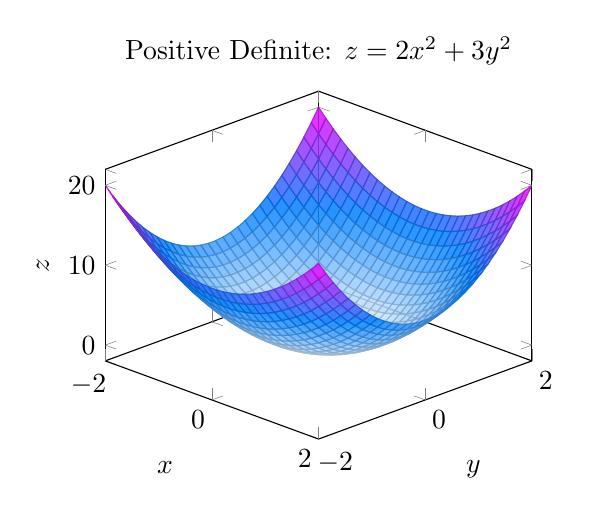
\begin{tikzpicture}
\begin{axis}[
  title={Positive Definite: \(z = 2x^2 + 3y^2\)},
  xlabel={\(x\)}, ylabel={\(y\)}, zlabel={\(z\)},
  width=7cm, height=6cm,
  colormap/cool,
  domain=-2:2, y domain=-2:2,
  samples=30,
  view={45}{30}
]
  \addplot3[surf, opacity=0.85] {2*x^2 + 3*y^2};
\end{axis}
\end{tikzpicture}
\hspace{1cm}
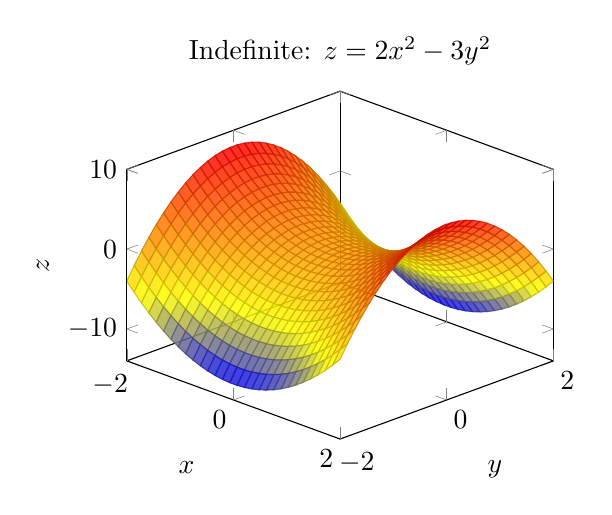
\begin{tikzpicture}
\begin{axis}[
  title={Indefinite: \(z = 2x^2 - 3y^2\)},
  xlabel={\(x\)}, ylabel={\(y\)}, zlabel={\(z\)},
  width=7cm, height=6cm,
  colormap/hot,
  domain=-2:2, y domain=-2:2,
  samples=30,
  view={45}{30}
]
  \addplot3[surf, opacity=0.85] {2*x^2 - 3*y^2};
\end{axis}
\end{tikzpicture}
\end{center}

\noindent The bowl shape of the PD surface confirms \(Q > 0\) everywhere except the
origin. The saddle of the indefinite form shows regions where \(Q > 0\) (ridges in
\(x\)-direction) and where \(Q < 0\) (valleys in \(y\)-direction).

%============================================================
% SECTION 5: Algorithmic Workflow
%============================================================
\section{Step-by-Step Algorithmic Workflow}

The following procedure converts any real symmetric matrix \(A\) into a complete
inertia classification.

\medskip
\begin{center}
\fbox{%
\begin{minipage}{0.88\textwidth}
\textbf{Algorithm: Classify a Quadratic Form via Rank, Index, Signature, and
Sylvester's Criterion}

\medskip
\textbf{Input:} Real symmetric \(n \times n\) matrix \(A\).\\
\textbf{Output:} Rank \(r\), index \(p\), signature \(s\), definiteness class.

\medskip
\begin{enumerate}[label=\textbf{Step \arabic*.}, leftmargin=*, nosep]
  \item \textbf{Find eigenvalues.}
        Solve \(\det(A - \lambda I) = 0\) to obtain
        \(\lambda_1, \lambda_2, \ldots, \lambda_n\) (with multiplicity).

  \item \textbf{Compute rank.}
        \[r = \#\{i : \lambda_i \neq 0\}.\]

  \item \textbf{Compute index.}
        \[p = \#\{i : \lambda_i > 0\}.\]

  \item \textbf{Compute signature.}
        \[q = r - p, \qquad s = p - q = 2p - r.\]

  \item \textbf{Apply Sylvester's criterion (verification / alternative).}
        Compute leading principal minors \(\Delta_1, \Delta_2, \ldots, \Delta_n\).
        \begin{itemize}[nosep]
          \item All \(\Delta_k > 0 \Rightarrow\) Positive Definite.
          \item \((-1)^k \Delta_k > 0\) for all \(k \Rightarrow\) Negative Definite.
          \item All \(\Delta_k \geq 0\) but some \(= 0 \Rightarrow\) Positive Semi-Definite
                (verify with eigenvalues).
          \item All \(\Delta_k \leq 0\) or \((-1)^k \Delta_k \geq 0\) with some
                \(= 0 \Rightarrow\) Negative Semi-Definite (verify with eigenvalues).
          \item Otherwise \(\Rightarrow\) Indefinite.
        \end{itemize}

  \item \textbf{Classify using the table.}
        Use the full classification table in Section 7.

  \item \textbf{State Sylvester's Law of Inertia (if applicable).}
        If a congruence transformation is involved, confirm that the computed
        \((r, p, s)\) for the transformed matrix matches those of the original.
\end{enumerate}
\end{minipage}%
}
\end{center}

%============================================================
% SECTION 6: Worked Numerical Examples
%============================================================
\section{Fully Worked Step-by-Step Numerical Examples}

\subsection*{Example 6.1 --- Rank, Index, and Signature of a \(3 \times 3\) Form}

Let
\[
A = \begin{pmatrix} 5 & 4 & 2 \\ 4 & 5 & 2 \\ 2 & 2 & 2 \end{pmatrix}.
\]

\textbf{Step 1: Characteristic polynomial.}
\[
\det(A - \lambda I) = 0.
\]
Computing:
\begin{align*}
\det(A - \lambda I)
&= (5-\lambda)\bigl[(5-\lambda)(2-\lambda) - 4\bigr]
 - 4\bigl[4(2-\lambda) - 4\bigr]
 + 2\bigl[8 - 2(5-\lambda)\bigr].
\end{align*}
Let us expand each bracket:
\[
(5-\lambda)(2-\lambda) - 4 = 10 - 7\lambda + \lambda^2 - 4 = \lambda^2 - 7\lambda + 6.
\]
\[
4(2-\lambda) - 4 = 8 - 4\lambda - 4 = 4 - 4\lambda.
\]
\[
8 - 2(5-\lambda) = 8 - 10 + 2\lambda = 2\lambda - 2.
\]
So:
\begin{align*}
\det(A - \lambda I)
&= (5-\lambda)(\lambda^2 - 7\lambda + 6) - 4(4 - 4\lambda) + 2(2\lambda - 2) \\
&= 5\lambda^2 - 35\lambda + 30 - \lambda^3 + 7\lambda^2 - 6\lambda - 16 + 16\lambda + 4\lambda - 4 \\
&= -\lambda^3 + 12\lambda^2 - 21\lambda + 10.
\end{align*}
Setting equal to zero and multiplying by \(-1\):
\[
\lambda^3 - 12\lambda^2 + 21\lambda - 10 = 0.
\]
Testing \(\lambda = 1\): \(1 - 12 + 21 - 10 = 0\). \quad \checkmark

Factor out \((\lambda - 1)\):
\[
\lambda^3 - 12\lambda^2 + 21\lambda - 10 = (\lambda - 1)(\lambda^2 - 11\lambda + 10)
= (\lambda - 1)(\lambda - 1)(\lambda - 10).
\]
Eigenvalues: \(\lambda_1 = 1\) (multiplicity 2), \(\lambda_2 = 10\).

\textbf{Step 2: Rank.}
All three eigenvalues are non-zero: \(r = 3\).

\textbf{Step 3: Index.}
All eigenvalues are positive (\(1, 1, 10\)): \(p = 3\).

\textbf{Step 4: Signature.}
\(q = 3 - 3 = 0\), so \(s = 3 - 0 = 3\).

\textbf{Step 5: Conclusion.}
\(r = 3,\; p = 3,\; s = 3\). Since \(p = n = 3\), the form is
\textbf{positive definite}. Canonical form: \(y_1^2 + y_2^2 + 10y_3^2\) (via orthogonal
diagonalisation, with eigenvalue scaling).

%------------------------------------------------------------
\subsection*{Example 6.2 --- Sylvester's Criterion on a \(3 \times 3\) Matrix}

Let
\[
D = \begin{pmatrix} 2 & -1 & 0 \\ -1 & 4 & -2 \\ 0 & -2 & 6 \end{pmatrix}.
\]

\textbf{Step 1: \(\Delta_1\).}
\[\Delta_1 = 2 > 0. \quad \checkmark\]

\textbf{Step 2: \(\Delta_2\).}
\[
\Delta_2 = \det\begin{pmatrix}2 & -1 \\ -1 & 4\end{pmatrix}
= (2)(4) - (-1)(-1) = 8 - 1 = 7 > 0. \quad \checkmark
\]

\textbf{Step 3: \(\Delta_3 = \det(D)\).}

Expanding along the first row:
\[
\det(D) = 2\det\begin{pmatrix}4 & -2 \\ -2 & 6\end{pmatrix}
- (-1)\det\begin{pmatrix}-1 & -2 \\ 0 & 6\end{pmatrix}
+ 0
\]
\[
= 2(24 - 4) + 1(-6 - 0) = 2(20) - 6 = 40 - 6 = 34 > 0. \quad \checkmark
\]

\textbf{Step 4: Conclusion.}
All three leading principal minors are positive (\(2, 7, 34\)).
By Sylvester's criterion, \(D\) is \textbf{positive definite}.

%------------------------------------------------------------
\subsection*{Example 6.3 --- Engineering Application: Testing a Lyapunov Matrix}

A control engineer designs a state-feedback controller for a second-order system.
The Lyapunov stability analysis yields the candidate symmetric matrix
\[
P = \begin{pmatrix} 6 & 2 \\ 2 & 3 \end{pmatrix}.
\]
Is \(V(\mathbf{x}) = \mathbf{x}^{T} P \mathbf{x}\) a valid Lyapunov function (i.e., is
\(P\) positive definite)?

\textbf{Step 1: Apply Sylvester's criterion.}
\[
\Delta_1 = 6 > 0. \quad \checkmark
\]
\[
\Delta_2 = \det\begin{pmatrix}6 & 2 \\ 2 & 3\end{pmatrix}
= 18 - 4 = 14 > 0. \quad \checkmark
\]

\textbf{Step 2: Confirm with eigenvalues.}
\[
\det(P - \lambda I) = (6-\lambda)(3-\lambda) - 4
= \lambda^2 - 9\lambda + 18 - 4 = \lambda^2 - 9\lambda + 14 = 0.
\]
\[
\lambda = \frac{9 \pm \sqrt{81 - 56}}{2} = \frac{9 \pm 5}{2}.
\]
\(\lambda_1 = 7 > 0,\quad \lambda_2 = 2 > 0\). Both positive.

\textbf{Step 3: Compute inertia.}
\(r = 2,\; p = 2,\; q = 0,\; s = 2\).

\textbf{Step 4: Engineering conclusion.}
\(P\) is \textbf{positive definite}. Therefore \(V(\mathbf{x}) = \mathbf{x}^{T} P \mathbf{x}
> 0\) for all \(\mathbf{x} \neq \mathbf{0}\), and \(V\) is a valid Lyapunov function.
The closed-loop system can be certified as stable via this Lyapunov candidate.

%============================================================
% SECTION 7: Tabular Reference / Comparison
%============================================================
\section{Tabular Reference --- Definiteness Classification}

\begin{center}
\begin{tabular}{@{}p{2.8cm} p{3.5cm} p{3.5cm} p{2.3cm} p{2.8cm}@{}}
\toprule
\textbf{Class} &
\textbf{Eigenvalue Condition} &
\textbf{Sylvester Criterion} &
\textbf{Rank / Index} &
\textbf{Geometric Shape} \\
\midrule
Positive Definite (PD) &
  All \(\lambda_i > 0\) &
  All \(\Delta_k > 0\) &
  \(r = n,\; p = n\) &
  Bowl (elliptic paraboloid, opens up) \\
\addlinespace
Positive Semi-Definite (PSD) &
  All \(\lambda_i \geq 0\), \(\exists\,\lambda_i = 0\) &
  All \(\Delta_k \geq 0\), \(\Delta_n = 0\) &
  \(r < n,\; p = r\) &
  Trough (flat in at least one direction) \\
\addlinespace
Negative Definite (ND) &
  All \(\lambda_i < 0\) &
  \((-1)^k\Delta_k > 0\) for all \(k\) &
  \(r = n,\; p = 0\) &
  Bowl opens down \\
\addlinespace
Negative Semi-Definite (NSD) &
  All \(\lambda_i \leq 0\), \(\exists\,\lambda_i = 0\) &
  \((-1)^k\Delta_k \geq 0\), \(\Delta_n = 0\) &
  \(r < n,\; p = 0\) &
  Inverted trough \\
\addlinespace
Indefinite (IND) &
  Mixed signs among \(\lambda_i\) &
  Sign pattern of \(\Delta_k\) mixed &
  \(0 < p < r\) &
  Saddle surface \\
\bottomrule
\end{tabular}
\end{center}

\bigskip
\begin{center}
\begin{tabular}{@{}p{2.8cm} p{3.0cm} p{3.0cm} p{3.5cm}@{}}
\toprule
\textbf{Quantity} & \textbf{Definition} & \textbf{Range} & \textbf{Engineering Use} \\
\midrule
Rank \(r\) &
  \(\#\{\lambda_i \neq 0\}\) &
  \(0 \leq r \leq n\) &
  Effective degrees of freedom in structural stiffness \\
\addlinespace
Index \(p\) &
  \(\#\{\lambda_i > 0\}\) &
  \(0 \leq p \leq r\) &
  Number of stable modes in vibration analysis \\
\addlinespace
Signature \(s\) &
  \(p - (r-p) = 2p - r\) &
  \(-r \leq s \leq r\) &
  Net stability balance in Lyapunov analysis \\
\addlinespace
Inertia triple &
  \((p,\, r-p,\, n-r)\) &
  sums to \(n\) &
  Complete invariant under congruence (Sylvester) \\
\bottomrule
\end{tabular}
\end{center}

%============================================================
% SECTION 8: Common Mistakes
%============================================================
\section{Common Student Mistakes and Pitfalls}

\begin{mistakebox}[Common Errors --- Rank, Index, Signature, and Definite Forms]
\begin{tabular}{@{}p{3.2cm} p{5.0cm} p{6.2cm}@{}}
\toprule
\textbf{Sub-Topic} & \textbf{Mistake} & \textbf{Correction} \\
\midrule
Rank &
  Confusing rank of \(A\) with the number of variables \(n\). &
  Rank equals the number of \emph{non-zero} eigenvalues. A full-rank form has
  \(r = n\), but rank can be less if some eigenvalues are zero. \\
\addlinespace
Rank &
  Using row-reduction rank without checking whether \(A\) is symmetric first. &
  Verify that the given matrix is symmetric (\(A = A^T\)) before applying
  spectral / eigenvalue methods. \\
\addlinespace
Index &
  Counting the index \(p\) as the number of \emph{negative} eigenvalues
  instead of \emph{positive} ones. &
  Index \(p\) counts \emph{positive} eigenvalues. The number of negative
  eigenvalues is \(q = r - p\). \\
\addlinespace
Signature &
  Writing \(s = p + q\) instead of \(s = p - q\). &
  Signature is \(s = p - q\). The sum \(p + q = r\) (rank), not the signature. \\
\addlinespace
Sylvester's Law &
  Thinking that congruent matrices must have the same eigenvalues. &
  Congruent matrices share rank, index, and signature --- but \emph{not}
  eigenvalues in general. Similarity preserves eigenvalues; congruence does not. \\
\addlinespace
Sylvester's Law &
  Applying Sylvester's Law to orthogonally similar matrices and assuming
  congruence. &
  Orthogonal similarity (\(B = P^T A P\) with \(P^T = P^{-1}\)) is a special
  case of congruence, but general congruence \(B = P^T A P\) does not require
  \(P\) to be orthogonal. \\
\addlinespace
Definite Forms &
  Testing only \(\Delta_n = \det(A) > 0\) and concluding positive definite. &
  Sylvester's criterion requires \emph{all} leading principal minors to be
  positive, not just the last one. \\
\addlinespace
Definite Forms &
  Confusing PSD with PD: if \(\det(A) = 0\) but all other \(\Delta_k > 0\),
  concluding the form is positive definite. &
  \(\det(A) = 0\) means \(A\) is singular and the form is at most positive
  \emph{semi-}definite, not strictly positive definite. \\
\bottomrule
\end{tabular}
\end{mistakebox}

%============================================================
% SECTION 9: Assessment Suite
%============================================================
\section{Comprehensive Assessment Suite}

\subsection*{9.1 Viva-Voce Questions}

\begin{enumerate}[label=\textbf{V\arabic*.}, leftmargin=*]
  \item \textbf{(Rank)} Define the rank of a quadratic form. How is it related to the
        eigenvalues of the associated symmetric matrix, and what does it mean geometrically
        when the rank is less than \(n\)?

  \item \textbf{(Rank)} If the matrix associated with a quadratic form has two zero
        eigenvalues and three non-zero eigenvalues, what is the rank of the form? What does
        this imply about the canonical form?

  \item \textbf{(Index)} Distinguish clearly between the rank and the index of a quadratic
        form. Can the index ever exceed the rank? Justify your answer.

  \item \textbf{(Signature)} A quadratic form in four variables has rank 3, index 2.
        Compute the signature and identify whether the form is positive semi-definite,
        negative semi-definite, or indefinite.

  \item \textbf{(Sylvester's Law)} State Sylvester's Law of Inertia. Why is invariance of
        the inertia triple under congruence transformations important in engineering
        applications?

  \item \textbf{(Sylvester's Law)} Two \(4 \times 4\) real symmetric matrices \(A\) and
        \(B\) satisfy \(B = P^T A P\) for some non-singular \(P\). Matrix \(A\) has
        eigenvalues \(3, 1, -2, -5\). What are the rank, index, and signature of \(B\)?

  \item \textbf{(Definite Forms)} Explain Sylvester's criterion for positive definiteness.
        Why is it sufficient to check only the leading principal minors and not all possible
        principal minors?

  \item \textbf{(Definite Forms)} A symmetric matrix has \(\Delta_1 = 5 > 0\),
        \(\Delta_2 = 3 > 0\), \(\Delta_3 = -7 < 0\). What is the definiteness
        classification? Is the matrix positive definite?

  \item \textbf{(Definite Forms)} In the context of Lyapunov stability, why must the matrix
        \(P\) in the candidate Lyapunov function \(V(\mathbf{x}) = \mathbf{x}^T P \mathbf{x}\)
        be positive definite rather than merely positive semi-definite?

  \item \textbf{(Mixed)} A \(3 \times 3\) symmetric matrix has eigenvalues
        \(\lambda_1 = 0,\; \lambda_2 = 4,\; \lambda_3 = -2\). Find its rank, index,
        signature, and definiteness class.
\end{enumerate}

\subsection*{9.2 Descriptive Exam Questions}

\begin{enumerate}[label=\textbf{D\arabic*.}, leftmargin=*]
  \item For the quadratic form
        \(Q = 6x_1^2 + 3x_2^2 + 14x_3^2 + 4x_1 x_2 + 18x_1 x_3 + 4x_2 x_3\),
        write down the associated symmetric matrix \(A\), find its eigenvalues,
        and determine the rank, index, and signature of \(Q\).
        \textit{Hint:} The matrix is
        \(A = \begin{pmatrix} 6 & 2 & 9 \\ 2 & 3 & 2 \\ 9 & 2 & 14 \end{pmatrix}\).
        Reduce and classify.

  \item State Sylvester's Law of Inertia. Given
        \(A = \begin{pmatrix} 4 & 2 \\ 2 & 3 \end{pmatrix}\) and the non-singular matrix
        \(P = \begin{pmatrix} 1 & 1 \\ 0 & 2 \end{pmatrix}\), compute \(B = P^T A P\),
        find the eigenvalues of both \(A\) and \(B\), and verify that rank, index, and
        signature are preserved under this congruence transformation.

  \item For the symmetric matrix
        \(M = \begin{pmatrix} 2 & 1 & 0 \\ 1 & 5 & -1 \\ 0 & -1 & 3 \end{pmatrix}\),
        apply Sylvester's criterion by computing all three leading principal minors.
        State the definiteness classification with full justification, and verify by
        finding the eigenvalues.

  \item For the control system with Lyapunov candidate matrix
        \(P = \begin{pmatrix} 8 & -2 & 0 \\ -2 & 5 & 1 \\ 0 & 1 & 4 \end{pmatrix}\),
        verify whether \(P\) is positive definite using Sylvester's criterion.
        Compute all leading principal minors, state the definiteness class, and explain
        the engineering implication for the stability of the system.

  \item Consider the indefinite quadratic form
        \(Q = 3x_1^2 - 2x_2^2 + x_3^2 - 4x_1 x_3\).
        Find the associated matrix \(A\), its eigenvalues, rank, index, and signature.
        Sketch (or describe) the shape of the surface \(z = Q\) in \(\mathbb{R}^3\) and
        explain what the indefiniteness means in a structural mechanics context (second
        variation of potential energy).
\end{enumerate}

\subsection*{9.3 Multiple Choice Questions}

\begin{enumerate}[label=\textbf{MCQ\arabic*.}, leftmargin=*]

  \item \textbf{(Rank)} The rank of the quadratic form associated with the matrix
        \(\begin{pmatrix} 1 & 0 & 0 \\ 0 & 3 & 0 \\ 0 & 0 & 0 \end{pmatrix}\) is:
        \begin{enumerate}[label=(\alph*), noitemsep]
          \item 0 \quad (b) 1 \quad \textbf{(c) 2} \quad (d) 3
        \end{enumerate}
        \textit{Explanation:} Two eigenvalues are non-zero (\(1\) and \(3\)); one is zero.
        Rank = 2.

  \item \textbf{(Index)} A real quadratic form has eigenvalues \(-5, -2, 4, 7\).
        The index of the form is:
        \begin{enumerate}[label=(\alph*), noitemsep]
          \item 0 \quad (b) 1 \quad \textbf{(c) 2} \quad (d) 4
        \end{enumerate}
        \textit{Explanation:} Two eigenvalues are positive (\(4\) and \(7\)), so \(p = 2\).

  \item \textbf{(Signature)} For eigenvalues \(-3, 2, 6\), the signature of the quadratic
        form is:
        \begin{enumerate}[label=(\alph*), noitemsep]
          \item \(-3\) \quad \textbf{(b) \(1\)} \quad (c) \(3\) \quad (d) \(2\)
        \end{enumerate}
        \textit{Explanation:} \(r = 3,\; p = 2,\; q = 1,\; s = 2 - 1 = 1\).

  \item \textbf{(Sylvester's Law)} If \(B = P^T A P\) for non-singular \(P\) and \(A\) is
        positive definite, then \(B\) is:
        \begin{enumerate}[label=(\alph*), noitemsep]
          \item Negative definite \quad \textbf{(b) Positive definite}
          \quad (c) Indefinite \quad (d) Positive semi-definite
        \end{enumerate}
        \textit{Explanation:} Congruence preserves rank, index, signature. PD means all
        eigenvalues \(> 0\), equivalently \(p = n\). This is invariant under congruence.

  \item \textbf{(Definite Forms)} A symmetric matrix \(A\) with leading principal minors
        \(\Delta_1 = 4,\; \Delta_2 = 7,\; \Delta_3 = 15\) is:
        \begin{enumerate}[label=(\alph*), noitemsep]
          \item Negative definite \quad (b) Indefinite
          \quad \textbf{(c) Positive definite} \quad (d) Positive semi-definite
        \end{enumerate}
        \textit{Explanation:} All leading principal minors are strictly positive, so
        Sylvester's criterion confirms positive definiteness.

  \item \textbf{(Definite Forms)} Which of the following conditions correctly identifies
        a \textbf{negative definite} \(3 \times 3\) symmetric matrix via Sylvester's
        criterion?
        \begin{enumerate}[label=(\alph*), noitemsep]
          \item \(\Delta_1 > 0,\; \Delta_2 > 0,\; \Delta_3 > 0\)
          \item \(\Delta_1 < 0,\; \Delta_2 < 0,\; \Delta_3 < 0\)
          \textbf{(c) \(\Delta_1 < 0,\; \Delta_2 > 0,\; \Delta_3 < 0\)}
          \item \(\Delta_1 > 0,\; \Delta_2 < 0,\; \Delta_3 > 0\)
        \end{enumerate}
        \textit{Explanation:} Negative definite requires \((-1)^k \Delta_k > 0\):
        \(\Delta_1 < 0,\;\Delta_2 > 0,\;\Delta_3 < 0\).

  \item \textbf{(Rank and Index)} A quadratic form in 5 variables has rank 4 and index 3.
        The number of negative eigenvalues is:
        \begin{enumerate}[label=(\alph*), noitemsep]
          \item 3 \quad \textbf{(b) 1} \quad (c) 2 \quad (d) 4
        \end{enumerate}
        \textit{Explanation:} \(q = r - p = 4 - 3 = 1\). One negative eigenvalue.

\end{enumerate}

%============================================================
% SECTION 10: Quick Recap and Formula Sheet
%============================================================
\section{Quick Recap and Formula Sheet}

\begin{learnbox}[Formula Sheet --- Rank, Index, Signature, and Definite Forms]
\begin{itemize}[noitemsep]
  \item \textbf{Rank:} \(r = \operatorname{rank}(A) = \#\{\lambda_i \neq 0\}\);
        equals the number of non-zero terms in the canonical form
        \(\displaystyle\sum_{i=1}^{r} d_i z_i^2\).

  \item \textbf{Index:} \(p = \#\{\lambda_i > 0\}\); counts the positive squared terms
        in the canonical form; range: \(0 \leq p \leq r\).

  \item \textbf{Signature:} \(s = p - q = 2p - r\) where \(q = r - p\) counts the
        negative eigenvalues; range: \(-r \leq s \leq r\).

  \item \textbf{Sylvester's Law of Inertia:} \(A \sim_{\text{congruence}} B\)
        \(\iff\) they share the same inertia triple \((p,\, q,\, n-r)\);
        eigenvalues are \emph{not} necessarily preserved.

  \item \textbf{Sylvester's Criterion (PD):}
        \(A\) is positive definite \(\iff\) all leading principal minors
        \(\Delta_1, \Delta_2, \ldots, \Delta_n > 0\).

  \item \textbf{Sylvester's Criterion (ND):}
        \(A\) is negative definite \(\iff\) \((-1)^k \Delta_k > 0\) for every
        \(k = 1, \ldots, n\).

  \item \textbf{Classification shortcut (eigenvalues):}
        PD: all \(\lambda_i > 0\); ND: all \(\lambda_i < 0\); PSD: all \(\lambda_i \geq 0\);
        NSD: all \(\lambda_i \leq 0\); Indefinite: mixed signs.

  \item \textbf{Lyapunov connection:} \(V(\mathbf{x}) = \mathbf{x}^T P \mathbf{x}\) is a
        valid Lyapunov function proving asymptotic stability \(\iff\) \(P\) is positive
        definite; verify via Sylvester's criterion or eigenvalue positivity.
\end{itemize}
\end{learnbox}

\end{document}
